%\documentclass[twocolumn,amsmath,amssymb]{revtex4}
\documentclass[preprint,amsmath,amssymb]{revtex4}
\usepackage{graphicx}
\usepackage{color}
\usepackage{amsmath}
\newcommand{\pd}[0]{\partial}
\newcommand{\pr}[1]{#1^{\prime}}
\newcommand\given[1][]{\:#1\vert\:}
\newcommand*\diff{\mathop{}\!\mathrm{d}}
\newcommand*\Diff[1]{\mathop{}\!\mathrm{d^#1}}

\begin{document}
\title{CBAMF -- Colloids Bayesian Augmented Monte Carlo Featuring}
\author{Matthew Bierbaum}
\author{Brian Leahy}
\author{Alexander Alemi}
\author{Neil Y.C. Lin}
\author{Itai Cohen}
\author{James P. Sethna}
\affiliation{Department of Physics, Cornell University, Ithaca, New York 14853}

\date{\today}

\maketitle

\section{BAMF -- Bayesian inference and Monte Carlo integration}

Here, we present an alternative method that does not require directly
featuring the particles (finding their positions) then finding and dealing
with the noise in those positional measurements.  Instead, we do a direct
integration over the noise using a generative model of the image data itself.

Let's assume we want to measure the fabric tensor as defined by a probability
distribution of configuration of particles. We can do so by the integration
of a general function $f$,

\begin{align*}
    \langle f(\vec{x}^{\alpha}, \vec{\theta})\rangle_{P(\vec{x}^{\alpha},\vec{\theta})} &= \int f(\vec{x}^{\alpha}, \vec{\theta}) P(\vec{x}^\alpha,\vec{\theta}) d\vec{x}^\alpha d\vec{\theta} \\
                                                                                        &\approx \frac{1}{N}\sum_{n} f(\vec{x}^\alpha, \vec{\theta})
\end{align*}
which we can sample via Monte Carlo.  However, how do we determine the
probability distribution from which to sample.  We turn to Baye's theorem for
the posterior probability given by a generative model for confocal images.
That is, we can sample from

\begin{equation}
    P(\vec{x}^\alpha, \vec{\theta} \given I^0_{ij}) \propto P(I^0_{ij} \given \vec{x}^\alpha, \vec{\theta}) P(\vec{\theta} \given \vec{x}^\alpha) P(\vec{x}^\alpha)
\end{equation}

The simplest way to sample this data is to use Metropolis-Hastings in which we
create a new sample according to some process and accept the move with
probability

\begin{equation}
    p = \rm{min}\left(\frac{P(\vec{x}_2, \vec{\theta}_2) g((\vec{x}_2,\vec{\theta}_2) \rightarrow (\vec{x}_1, \vec{\theta}_1))}{P(\vec{x}_1, \vec{\theta}_1) g((\vec{x}_1,\vec{\theta}_1) \rightarrow (\vec{x}_2, \vec{\theta}_2))}, 1\right)
\end{equation}
where $P$ is the likelihood function from earlier and $g$ is the probability of
our sampling process.  Given that these are accurately calculated, we can
satisfy detailed balance and properly sample our posterior probability for MC.
What is this process for choosing these samples?  In the simplest case, we can
just choose random positions uniformly, but this would at best provide horrible
convergence.  Instead, we choose to sample using N-body dynamics which respect
our priors on particle configurations.

\subsection{Generative model}

To get the answer, we need to have a generative model for the image which
includes as a subset, the true model from which the data was made.  To this
end, we have to understand how our data was generated from physics / optics /
image processing / etc.  Our model as we are building it will include:

\begin{itemize}

    \item {\bf Colloids are spheres} -- We will convolve with a disc to
        generate the platonic colloid particle

    \item {\bf Spheres aren't perfect} -- Each particle is subject to a slight
        (or intentional polydispersity) size variation, as well as ellipticity

    \item {\bf CCDs have noise} -- CCDs have shot noise which add randomness to
        the data that comes back as an image

    \item {\bf Microscopes are hard} -- The optics and illumination create an
        effective PSF which modifies how the data comes back from the platonic
        structure

    \item {\bf Lenses are dusty} -- There is random (but systematic) noise due
        to dust, variations in coverslip, lens, etc.

\end{itemize}

\subsection{Colloids are spheres}

To model the colloids as spheres, we will be going into Fourier space to
generate platonic models of them in the optical system.  We denote the image as
$I(\vec{x})$ and the particle positions as $\{\vec{x}^{\alpha}\}$ with radii
$\{r^{\alpha}\}$.  We can generate our image using Fourier methods by knowing that
in $N$-dimensions, the Fourier transform of a unit sphere is given by

\begin{align*}
    \Pi(k) &= \frac{J_{d/2}(k)}{k^{d/2}} & d\,\,\rm{even} \\
           &= \sqrt{\frac{2}{\pi}}\, \frac{j_{(d-1)/2}(k)}{k^{(d-1)/2}} &d\,\,\rm{odd}
\end{align*}

where $J_n$ are Bessel functions of the first kind and $j_n$ are Spherical
Bessel functions of the first kind.  The relevant functions for our purposes
are

\begin{align*}
    j_0(x) &= \frac{\sin{x}}{x} \\
    j_1(x) &= \frac{\sin{x}}{x^2} - \frac{\cos{x}}{x} \\
    J_1(x) &= \sum_{m=0}^{\infty} \frac{(-1)^m}{m!\,\Gamma(m+2)} \left(\frac{x}{2}\right)^{2m+1}
\end{align*}

where $j_0$ is used for $d=1$, $j_1$ for $d=3$, and $J_1$ for $d=2$.  Once we
have this function for the sphere, we take also need to account for radii which
are not exactly $1$, and so we arrive at the following explicit form for the
radial portion of the shape function (defining $q = 2\pi k R$)

\begin{align*}
    \Pi_{d=1}(q,R) &= 2 R \,\frac{\sin{q}}{q} \\
    \Pi_{d=2}(q,R) &= 2 \pi R^2 \,\frac{J_1(q)} {q} \\
    \Pi_{d=3}(q,R) &= \frac{4\pi R^3}{q}\left(\frac{\sin{q}}{q} -\cos{q}\right) 
\end{align*}

\begin{align*}
    I(x) &= \sum_{\alpha} \int \diff x^{\prime}\, \Pi(\vec{x} - \vec{x}^{\prime}, r^{\alpha}) \,\delta(\vec{x}^{\prime} - \vec{x}^{\alpha}) \\
         &= \sum_{\alpha} \int \diff x^{\prime} \diff k \diff q\, \Pi(k) e^{i \vec{k} \cdot ( \vec{x} - \vec{x}^{\prime})} e^{i \vec{q} \cdot (\vec{x}^{\prime} - \vec{x}^{\alpha})} \\
         &= \sum_{\alpha} \int \diff x^{\prime} \diff k \diff q\, \Pi(k, r^{\alpha}) e^{i \vec{x}^{\prime} \cdot ( \vec{q} - \vec{k})} e^{- i \vec{q} \cdot \vec{x}^{\alpha}} e^{i \vec{k} \cdot \vec{x}} \\
         &= \sum_{\alpha} \int \diff k\, \Pi(k, r^{\alpha}) e^{ - i \vec{k} \cdot \vec{x}^{\alpha}} e^{ i \vec{k} \cdot \vec{x}}
\end{align*}

which is the plane-wave translated sphere at every place that a particle
appears. From this, we are able to accurately construct the true image of
particles on a small grid using Fourier methods due to the fast convergence
provided by $k$-space representations.

\begin{figure}[ht]
    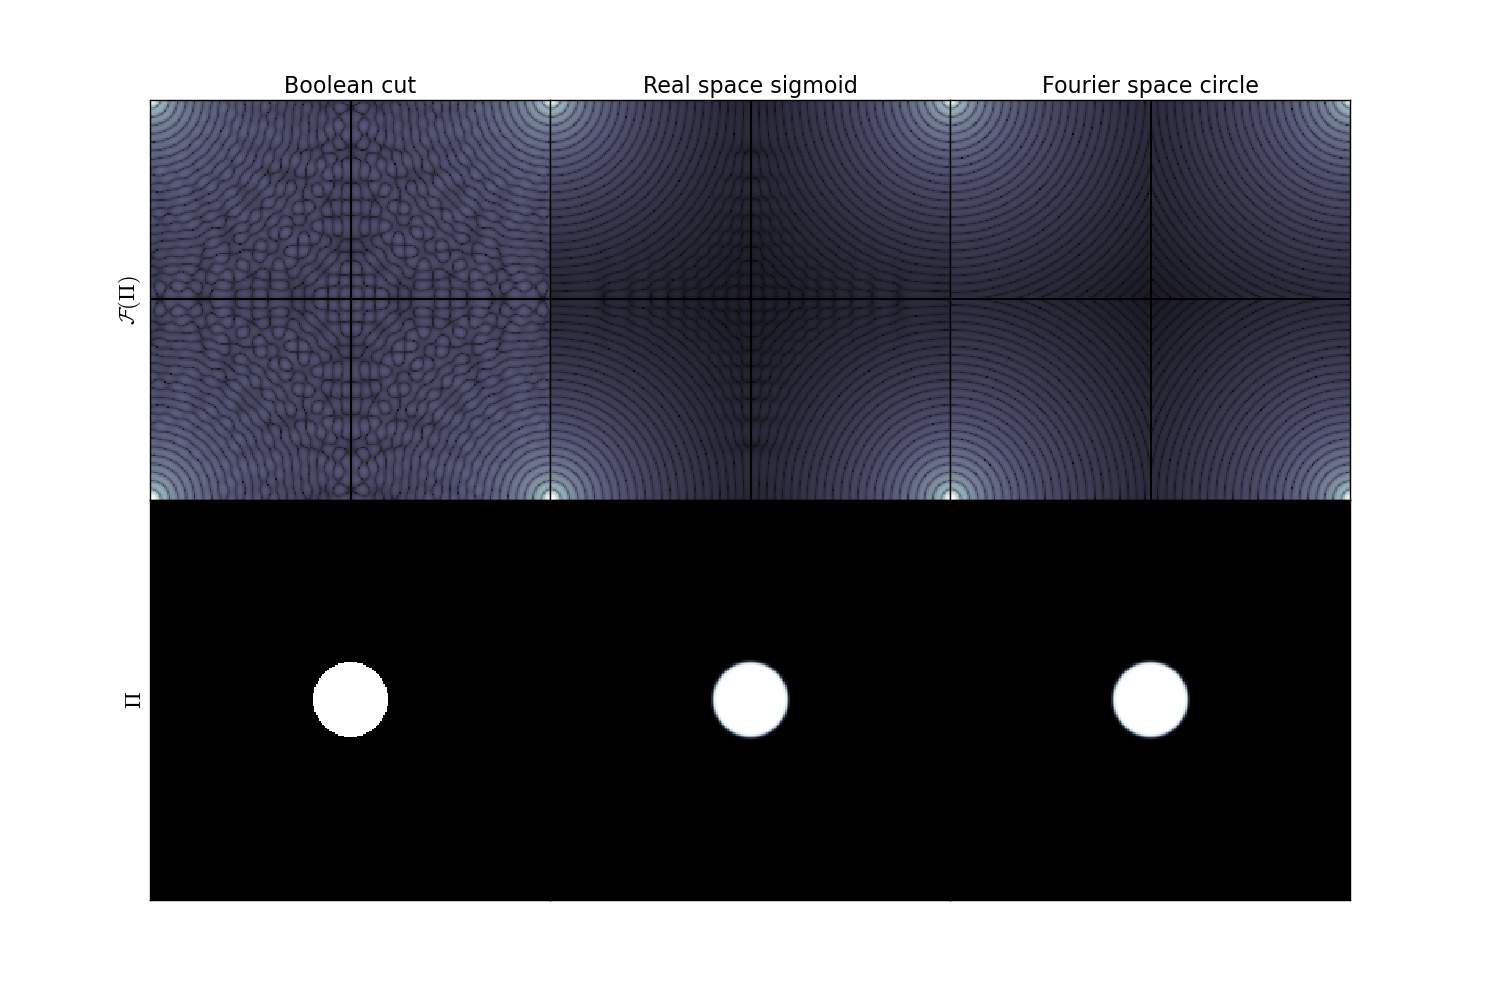
\includegraphics[width=0.95\columnwidth]{figs/sphere_generation_comparison.png}

    \caption{A comparison of different methods to create an image of a sphere.
        These methods are (left) making a boolean cut as a function of the
        distance from the center (middle) using a sigmoidal function $\Pi(r) =
        (1 + e^{-\alpha r_0}) / (1 + e^{\alpha (r - r_0)})$ and (right) using the Fourier shape
    generation described in this section.}

    \label{fig:sphere_generation_comparison}
\end{figure}



\subsection{CCDs have noise}

We generate our true image, we must also include intrinsic shot noise.
Theoretically, this type of noise is the only part of the confocal image
that we will not be able to reconstruct in any way.  In particular, it
will be the noise distribution that we use to create our likelihood function
meaning given a hyperparameter which describes its distribution.

To make this noise, at the last step of the image generation process, we
add a random field to the CCD,

\begin{equation}
    I(\vec{x}) = I(\vec{x}) + N(\vec{x}, \mu, \sigma)
\end{equation}

where $\langle N(\vec{x}^a_i, \mu, \sigma) N(\vec{x}^b_j, \mu, \sigma)\rangle =
\delta^{ab} \delta_{ij}$ and $\sigma$ determines the standard deviation of that
noise.

\section{Spatially varying PSF}

Given we have a PSF $P$ and illumination field, platonic sphere combination of
$S$, the combined image can be obtained by convolution.  For this simple look
at spatially varying PSFs, let's look at a gaussian in $\rho$, $z$ where the
dependence on $\rho$ does not change with height, but $z$ does.

\begin{align*}
    I(x) &= \int P(\pr{x}; x) S(x - \pr{x}) \diff \pr{x} \\
         &= \int \frac{1}{(2\pi)^{3/2} \sigma_x\sigma_y\sigma_z(z)} \exp\left(\frac{-\pr{x}^2}{2\sigma_x^2} + \frac{-\pr{y}^2}{2\sigma_y^2}\right) \exp\left(\frac{-\pr{z}^2}{2\sigma_z(z)^2}\right) S(\vec{x}-\pr{\vec{x}}) \diff \pr{x} \diff \pr{y} \diff \pr{z}
\end{align*}

Let's assume that the PSF behaves such that $\sigma_z(z) = \sigma_z f(z)$ where
$f(z)$ can probably be as simple as $f(z) = 1 + z/z_0$.  Substituting this back
into the expression

\begin{align*}
    I(\vec{x}) &= \int \frac{1}{(2\pi)^{3/2} \sigma_x\sigma_y\sigma_z} \exp\left(\frac{-\pr{x}^2}{2\sigma_x^2} + \frac{-\pr{y}^2}{2\sigma_y^2}\right) \exp\left(\frac{-\pr{z}^2}{2\sigma_z^2}\right) S(\vec{x}-\pr{\vec{x}}) \frac{e^{-1/f^2(z)}}{f(z)} \diff \pr{x} \diff \pr{y} \diff \pr{z}
\end{align*}


\bibliography{references}

\end{document}
